\documentclass{article}
\usepackage[utf8]{inputenc}
\usepackage[margin=1.125in]{geometry}
\usepackage{listings}
\usepackage{amsmath}
\usepackage{graphicx}
\usepackage{xcolor}
\usepackage{inconsolata}
\graphicspath{{img/}}
\lstset{ 
  backgroundcolor=\color{white},   % choose the background color; you must add \usepackage{color} or \usepackage{xcolor}; should come as last argument
  basicstyle=\ttfamily\footnotesize,            % the size of the fonts that are used for the code
  breakatwhitespace=false,         % sets if automatic breaks should only happen at whitespace
  breaklines=true,                 % sets automatic line breaking
  commentstyle=,    % comment style
  deletekeywords={...},            % if you want to delete keywords from the given language
  keepspaces=true,                 % keeps spaces in text, useful for keeping indentation of code (possibly needs columns=flexible)
  keywordstyle=\bfseries,         % keyword style
  language=Java,                   % the language of the code
  morekeywords={*,...},            % if you want to add more keywords to the set
  showspaces=false,                % show spaces everywhere adding particular underscores; it overrides 'showstringspaces'
  showstringspaces=false,          % underline spaces within strings only
  showtabs=false,                  % show tabs within strings adding particular underscores
  stepnumber=2,                    % the step between two line-numbers. If it's 1, each line will be numbered
  stringstyle=,     % string literal style
  tabsize=2,	                   % sets default tabsize to 2 spaces
  xleftmargin=0.5cm
}

\title{50.003 Elements of Software Construction\\Final Exam Toolbox}
\author{Joel Huang}
\date{\today}

\begin{document}

\maketitle

\section{Software Design Patterns}
\subsection{Factory Design Pattern}
Factory pattern is one of the most used design patterns in Java. This type of design pattern comes under creational pattern as this pattern provides one of the best ways to create an object.\\\\
In Factory pattern, we create object without exposing the creation logic to the client and refer to newly created object using a common interface.
\lstinputlisting{src/PizzaStore.java}
\break

\subsection{Observer Design Pattern}
Observer pattern is used when there is one-to-many relationship between objects such as if one object is modified, its dependent objects are to be notified automatically.
\lstinputlisting{src/ObserverPattern.java}
\break

\subsection{Decorator Design Pattern}
Decorator pattern allows a user to add new functionality to an existing object without altering its structure. This type of design pattern comes under structural pattern as this pattern acts as a wrapper to existing class.\\\\
This pattern creates a decorator class which wraps the original class and provides additional functionality keeping class methods signature intact.
\lstinputlisting{src/DecoratorDemo.java}
\break

\subsection{Strategy Design Pattern}
In Strategy pattern, a class behavior or its algorithm can be changed at run time. This type of design pattern comes under behavior pattern.\\\\
In Strategy pattern, we create objects which represent various strategies and a context object whose behavior varies as per its strategy object. The strategy object changes the executing algorithm of the context object.\\
\lstinputlisting{src/StrategyPattern.java}
\break

\subsection{Visitor Design Pattern}
In Visitor pattern, we use a visitor class which changes the executing algorithm of an element class. Execution of elements can vary as and when visitor varies. As per the pattern, element object has to accept the visitor object so that visitor object handles the operation on the element object.
\lstinputlisting{src/VisitorPatternOriginal.java}
\break

\section{Testing}
\subsection{JUnit Overview}
JUnit can be used to test an entire object, part of an object, a method or some interacting methods, and interaction between several objects. Test classes include a \textbf{test runner} to run the tests (main()), a collection of \textbf{test methods}, methods to \textbf{set up} the state before/\textbf{update} the state after each test and before and after all tests
\subsubsection{Assertions}
Each test method checks a condition (assertion) and reports to the test runner whether the test failed or succeeded. 
\begin{itemize}
\item \lstinline{assertTrue (String message, boolean condition)}
\item \lstinline{assertFalse (String message, boolean condition)}
\item \lstinline{assertEquals (Object expected, Object actual)}
    \begin{itemize}
        \item Asserts that two objects \textbf{are equal}.
    \end{itemize}
\item \lstinline{assertSame (Object expected, Object actual)}
    \begin{itemize}
        \item Asserts that two objects \textbf{refer} to the same object.
    \end{itemize}
\item \lstinline{assertNotSame (Object expected, Object actual)}
    \begin{itemize}
        \item Asserts that two objects \textbf{do not refer} to the same object.
    \end{itemize}
\item \lstinline{assertNull (Object object)}
\item \lstinline{assertNotNull (Object object)}
\item \lstinline{fail (String message)}
\end{itemize}

\subsubsection{Decorators}
Different tests can use the objects without sharing state. Objects used in test fixtures should be declared as \textbf{instance variables}. Here are some general rules:
\begin{itemize}
\item Using \lstinline{@Test}
    \begin{itemize}
        \item The Test annotation tells JUnit that the public void method to which it is attached can be run as a test case.
    \end{itemize}
\item Objects should be initialized in a \lstinline{@Before} method
    \begin{itemize}
        \item Several tests need similar objects created before they can run. Annotating a public void method with \lstinline{@Before} causes that method to be run before each Test method.
    \end{itemize}
\item Objects can be deallocated or reset in an \lstinline{@After} method
    \begin{itemize}
        \item If you allocate external resources in a \lstinline{@Before} method, you need to release them after the test runs. Annotating a public void method with \lstinline{@After} causes that method to be run after the Test method.
    \end{itemize}
\item \lstinline{@BeforeClass} and \lstinline{@AfterClass}: Annotating a public static void method with \lstinline{@BeforeClass} causes it to be run once before any of the test methods in the class. \lstinline{@AfterClass} will perform the method after all tests have finished. This can be used to perform clean-up activities.
\end{itemize}

\subsubsection{Parameterize your test}
Parameterized unit tests call the constructor for each logical set of data values. The same tests are then run on each set of data values.
\begin{enumerate}
    \item Annotate test class with \lstinline{@RunWith(Parameterized.class)}.
    \item Create a public static method annotated with \lstinline{@Parameters} that returns a Collection of Objects (as Array) as test data set.
    \item Create a public constructor that takes in what is equivalent to one "row" of test data.
    \item Create an instance variable for each "column" of test data.
    \item Create your test case(s) using the instance variables as the source of the test data.
\end{enumerate}
\lstinputlisting{src/ParameterizedTest.java}
\break

\subsection{Mocking objects}
Mocking is used to simulate objects that have not been implemented. For example if you have to make a network call, you manually hard-code/return the network response for ALL kinds of network responses and see if your app is working as you expect. You never assume/test a 200 with incorrect data, because that is not your responsibility. Your responsibility is to test your app with a correct 200, or in case of a 400, 500, you test if your app throws the right error.
\subsubsection{JMock mocking procedure}
\begin{enumerate}
    \item \lstinline{Mockery context = new Mockery();}
        \begin{itemize}
            \item Create a Mockery object. A Mockery represents the context of the object under test: the objects that it communicates with. A Mockery creates mock objects and checks expectations that are set upon those mock objects. By convention the Mockery is stored in an instance variable named context.
        \end{itemize}
    \item \lstinline{Turtle turtle = context.mock(Turtle.class);}
        \begin{itemize}
            \item NOTE: If a mock object is stored in a local variable, the variable must be declared as final so that it can be referred to from within expectation blocks.
        \end{itemize}
    \item \lstinline|context.checking(new Expectations() {{|\\
          \lstinline|  ... expectations go here ...|\\
          \lstinline|}});|\\
          \lstinline|... call code being tested ...|\\
          \lstinline|context.assertIsSatisfied();|
        \begin{itemize}
            \item An expectations block can contain any number of expectations. A test can contain multiple expectation blocks. Expectations in later blocks are appended to those in earlier blocks. Expectations can be interspersed with calls to the code under test.
            \item Invocation count:
            \begin{itemize}
                \item \lstinline{oneOf}	The invocation is expected once and once only.
                \item \lstinline{exactly(n).of}	The invocation is expected exactly n times. Note: one is a convenient shorthand for exactly(1).
                \item \lstinline{atLeast(n).of}	The invocation is expected at least n.
                \item \lstinline{atMost(n).of}	The invocation is expected at most n times.
                \item \lstinline{between(min, max).of}	The invocation is expected at least min times and at most max times.
                \item \lstinline{allowing}	The invocation is allowed any number of times but does not have to happen.
                \item \lstinline{ignoring}	The same as allowing. Allowing or ignoring should be chosen to make the test code clearly express intent.
                \item \lstinline{never}	The invocation is not expected at all. This is used to make tests more explicit and so easier to understand.
            \end{itemize}
            \item Actions:
            \begin{itemize}
                \item \lstinline{will(returnValue(v))}	Return v to the caller.
                \item \lstinline{will(returnIterator(c))}	Return a new iterator over collection c on each invocation.
                \item \lstinline{will(returnIterator(v1, v2, ..., vn))}	Return a new iterator over elements v1 to vn on each invocation.
                \item \lstinline{will(throwException(e))}	Throw e to the caller.
                \item \lstinline{will(doAll(a1, a2, ..., an))}	Do all actions a1 to an on every invocation.
                \item For example, \lstinline{oneOf (calculator).add(1, 1); will(returnValue(2));}
            \end{itemize}
            \item Sequences, for invocations in an order:
            \begin{itemize}
                \item \lstinline{final Sequence sequence-name = context.sequence("sequence-name");}\\
                      \lstinline{oneOf (turtle).forward(10); inSequence(drawing);}\\
                      \lstinline{oneOf (turtle).turn(45); inSequence(drawing);}
            \end{itemize}
        \end{itemize}
\end{enumerate}

\lstinputlisting{src/TestWithMock.java}
\break

\subsection{Fuzzing}
\subsubsection{Regular fuzzing}
\lstinputlisting{src/simple-fuzzer.c}
\break

\subsubsection{Mutation fuzzing}
Mutation fuzzing includes flipping a bit, trimming, swapping characters, and inserting characters.
\lstinputlisting{src/generalized_fuzzer.py}
\break

\subsection{Web Testing}
Selenium API allows access to the DOM and its content. Selected classes and methods:
\begin{enumerate}
    \item \lstinline{public interface WebElement}\\Represents an HTML element. Generally, all interesting operations to do with interacting with a page will be performed through this interface. All method calls will do a freshness check to ensure that the element reference is still valid. This essentially determines whether or not the element is still attached to the DOM. If this test fails, then an StaleElementReferenceException is thrown, and all future calls to this instance will fail.
        \begin{itemize}
            \item \lstinline{void clear()} If this element is a text entry element, this will clear the value.
            \item \lstinline{void click()} Click this element.
            \item \lstinline{WebElement findElement(By by)} Find the first WebElement using the given method.
            \item \lstinline{List<WebElement> findElements(By by)} Find all elements within the current context using the given mechanism.
            \item \lstinline{String getAttribute(String name)} Get the value of the given attribute of the element.
            \item \lstinline{String getCssValue(String propertyName)} Get the value of a given CSS property.
            \item \lstinline{Point getLocation()} Where on the page is the top left-hand corner of the rendered element?
            \item \lstinline{getRect()} Returns the location and size of the rendered element.
            \item \lstinline{Dimension getSize()} What is the width and height of the rendered element?
            \item \lstinline{String	getTagName()} Get the tag name of this element.
            \item \lstinline{String	getText()} Get the visible text.
            \item \lstinline{isDisplayed()} Is this element displayed or not? This method avoids the problem of having to parse an element's "style" attribute.
            \item \lstinline{boolean isEnabled()} Is the element currently enabled or not? This will generally return true for everything but disabled input elements.
            \item \lstinline{boolean isSelected()} Determine whether or not this element is selected or not.
            \item \lstinline{void sendKeys(CharSequence... keysToSend)} Use this method to simulate typing into an element, which may set its value.
            \item \lstinline{void submit()} If this current element is a form, or an element within a form, then this will be submitted to the remote server.
        \end{itemize}
    \item \lstinline{public interface WebDriver}\\The main interface to use for testing, which represents an idealised web browser. Key methods are \lstinline{get(String)}, which is used to load a new web page, and the various methods similar to \lstinline{findElement(By)}, which is used to find \lstinline{WebElements}.
        \begin{itemize}
            \item \lstinline{void close()} Close the current window, quitting the browser if it's the last window currently open.
            \item \lstinline{WebElement findElement(By by)} Find the first WebElement using the given method.
            \item \lstinline{List<WebElement> findElements(By by)} Find all elements within the current page using the given mechanism.
            \item \lstinline{void get(String url)} Load a new web page in the current browser window.
            \item \lstinline{String getCurrentUrl()} Get a string representing the current URL that the browser is looking at.
            \item \lstinline{String getPageSource()} Get the source of the last loaded page.
            \item \lstinline{String getTitle()} The title of the current page.
            \item \lstinline{String getWindowHandle()} Return an opaque handle to this window that uniquely identifies it within this driver instance.
            \item \lstinline{Set<String> getWindowHandles()} Return a set of window handles which can be used to iterate over all open windows of this WebDriver instance by passing them to switchTo().WebDriver.Options.window()
            \item \lstinline{WebDriver.Options manage()} Gets the Option interface
            \item \lstinline{WebDriver.navigate()} An abstraction allowing the driver to access the browser's history and to navigate to a given URL.
            \item \lstinline{void quit()} Quits this driver, closing every associated window.
            \item \lstinline{WebDriver.TargetLocator switchTo()} Send future commands to a different frame or window.
        \end{itemize}
    \item \lstinline{public interface ExpectedCondition<T>}\\Models a condition that might reasonably be expected to eventually evaluate to something that is neither null nor false. Examples would include determining if a web page has loaded or that an element is visible. Consider the Google login example. We do not need to wait always 10 seconds. We only need to wait until the password field becomes visible in the page.
            \begin{itemize}
                \item
                    \lstinline|try {|\\
                    \lstinline|  WebDriverWait wait = new WebDriverWait(driver, 10);|\\
                    \lstinline|  // wait only until the password element becomes visible|\\
                    \lstinline|  wait.until(ExpectedConditions.elementToBeClickable(By.name("password")));|\\
                    \lstinline|  // now locate the password field in the current page|\\
                    \lstinline|  WebElement password = driver.findElement(By.name("password"));|\\
                    \lstinline|  // send password|\\
                    \lstinline|  password.sendKeys(myPassword);|\\
                    \lstinline|  // login and :)|\\
                    \lstinline|  nextButton = driver.findElement(By.id("passwordNext"));|\\
                    \lstinline|  nextButton.click();|\\
                    \lstinline|} catch (Exception NoSuchElementException) {|\\
                    \lstinline|  System.out.println("login name invalid");|\\
                    \lstinline|}|
        \end{itemize}
\end{enumerate}
Random link clicking is implemented through WebDriver and clicking a random WebElement:
\lstinputlisting{src/ISTDWebsiteClickRandomLink.java}
\break

\section{Code Refactoring}
The more lines found in a method, the harder it is to figure out what the method does. This is the main reason for this refactoring. Besides eliminating rough edges in your code, extracting methods is also a step in many other refactoring approaches. Refactoring gives you more readable code, less code duplication. Often the code that is found in a method can be reused in other places in your program. Also isolates independent parts of code, meaning that errors are less likely (such as if the wrong variable is modified).
\subsection{Code smells}
\subsubsection{Long method}
\begin{itemize}
    \item As a rule of thumb, if you feel the need to comment on something inside a method, you should take this code and put it in a new method. Even a single line can and should be split off into a separate method, if it requires explanations. And if the method has a descriptive name, nobody will need to look at the code to see what it does.
    \item Solution: Extract method. Change from\\
        \lstinline|void printOwing() {|\\
        \lstinline|  printBanner();|\\\\
        \lstinline|  //print details|\\
        \lstinline|  System.out.println("name: " + name);|\\
        \lstinline|  System.out.println("amount: " + getOutstanding());|\\
        \lstinline|}|
    \item to:\\
        \lstinline|void printOwing() {|\\
        \lstinline|  printBanner();|\\
        \lstinline|  printDetails(getOutstanding());|\\
        \lstinline|}|\\
        \lstinline||\\
        \lstinline|void printDetails(double outstanding) {|\\
        \lstinline|  System.out.println("name: " + name);|\\
        \lstinline|  System.out.println("amount: " + outstanding);|\\
        \lstinline|}|
\end{itemize}

\subsubsection{Repeated code}
\begin{itemize}
    \item There is also more subtle duplication, when specific parts of code look different but actually perform the same job. This kind of duplication can be hard to find and fix. Sometimes duplication is purposeful. When rushing to meet deadlines and the existing code is "almost right" for the job, novice programmers may not be able to resist the temptation of copying and pasting the relevant code. And in some cases, the programmer is simply too lazy to de-clutter.
    \item Use the same approach as long method to solve it.
\end{itemize}

\subsubsection{Black Hole class/Large class}
\begin{itemize}
    \item As is the case with long methods as well, programmers usually find it mentally less taxing to place a new feature in an existing class than to create a new class for the feature. When a class is wearing too many (functional) hats, think about splitting it up.
    \item Single-responsibility classes are more reliable and tolerant of changes. For example, say that you have a class responsible for ten different things. When you change this class to make it better for one thing, you risk breaking it for the nine others.
    \item To solve this, create new classes. Create a relationship between the old class and the new one. Optimally, this relationship is unidirectional; this allows reusing the second class without any issues. Nonetheless, if you think that a two-way relationship is necessary, this can always be set up.
\end{itemize}

\subsubsection{Data class (Not to be confused with \textit{Data clump})}
\begin{itemize}
    \item A data class refers to a class that contains only fields and crude methods for accessing them (getters and setters). These are simply containers for data used by other classes. These classes do not contain any additional functionality and cannot independently operate on the data that they own.
    \item Fixing this improves understanding and organization of code. Operations on particular data are now gathered in a single place, instead of haphazardly throughout the code.
    \item After the class has been filled with well thought-out methods, you may want to get rid of old methods for data access that give overly broad access to the class data.
    \item Example:\\
        \lstinline|class Point3D {|\\
        \lstinline|  int x;|\\
        \lstinline|  int y;|\\
        \lstinline|  int z;|\\\\
        \lstinline|  public Point3D(int x, int y, int z) {|\\
        \lstinline|    this.x = x;|\\
        \lstinline|    this.y = y;|\\
        \lstinline|    this.z = z;|\\
        \lstinline|  }|\\
        \lstinline|  public void setX(int x) {this.x = x;}|\\
        \lstinline|  public void setY(int y) {this.y = y;}|\\
        \lstinline|  public void setZ(int z) {this.z = z;}|\\
        \lstinline|  public int getX(int x) {return x;}|\\
        \lstinline|  public int getY(int y) {return y;}|\\
        \lstinline|  public int getZ(int z) {return z;}|\\
        \lstinline|}|
\end{itemize}

\subsubsection{Data clump}
\begin{itemize}
    \item Sometimes different parts of the code contain similar groups of variables (such as parameters for connecting to a database). These clumps (e.g. arg1, arg2, arg3, ..., which are always found together) should be turned into a class of its own.
    \item If you want to make sure whether or not some data is a data clump, just delete one of the data values and see whether the other values still make sense. If this is not the case, this is a good sign that this group of variables should be combined into an object.
    \item Refactor from:\\
        \lstinline|void demoClump() {|\\
        \lstinline|  int param1 = 0;|\\
        \lstinline|  String param2 = "yes";|\\
        \lstinline|  boolean param3 = true;|\\
        \lstinline|  action (int p1, String p2, boolean p3);|\\
        \lstinline|}|\\
    \item to:\\
        \lstinline|class NotClumped {|\\
        \lstinline|  int param1 = 0;|\\
        \lstinline|  String param2 = "yes";|\\
        \lstinline|  boolean param3 = true;|\\
        \lstinline|  action () { // use vars here }|\\
        \lstinline|}|\\\\
        \lstinline|... then the class can be used as ...|\\
        \lstinline|NotClumped nc = new NotClumped(0, "yes", true);|\\
        \lstinline|nc.action();|\\
\end{itemize}

\subsubsection{Long parameter}
\begin{itemize}
    \item A long list of parameters might happen after several types of algorithms are merged in a single method. A long list may have been created to control which algorithm will be run and how.
    \item Solution is to only pass parameters that are needed. Let's say we are passing \lstinline{basePrice}, \lstinline{discountAmount}, and \lstinline{fees} to a method called \lstinline{discountedPrice()} which calculates the new discounted price. \lstinline{discountAmount} and \lstinline{fees} actually do not need to be passed in and can be obtained in the method itself.
\end{itemize}

\subsubsection{Shotgun surgery}
\begin{itemize}
    \item Making any modifications requires that you make many small changes to many different classes. This happens when a single responsibility has been split up among a large number of classes.
    \item Move methods and fields to force existing class behaviors into a single class. If there is no class appropriate for this, create a new one.
\end{itemize}

\subsubsection{Feature envy}
\begin{itemize}
    \item A method accesses the data of another object more than its own data. This smell may occur after fields are moved to a data class. If this is the case, you may want to move the operations on data to this class as well.
    \item Solve this by moving the methods from the envied class to the envious class.
    \item Example:\\
        \lstinline|class Project {|\\
        \lstinline|}|\\\\
        \lstinline|class GirlFriend {|\\
        \lstinline|  Project myProject;|\\
        \lstinline|  public GirlFriend(Project myProject) {this.myProject = myProject;}|\\
        \lstinline|  public Project getProject() {return this.myProject;}|\\
        \lstinline|}|\\\\
        \lstinline|public class LostInLove {|\\
        \lstinline|  GirlFriend myGirlfriend;|\\
        \lstinline|  Project myProject;|\\\\
        \lstinline|  public LostInLove(GirlFriend myGirlfriend, Project myProject) {|\\
        \lstinline|    this.myGirlfriend = myGirlfriend;|\\
        \lstinline|    this.myProject = myProject;|\\
        \lstinline|  }|\\\\
        \lstinline|  public void doHerProject() {|\\
        \lstinline|    Project herProject = myGirlfriend.getProject();|\\
        \lstinline|    workOnProject(herProject);|\\
        \lstinline|  }|\\\\
        \lstinline|  public void doProject() {workOnProject(myProject);}|\\\\
        \lstinline|  public void workOnProject(Project p) {}|\\
        \lstinline|}|
\end{itemize}

\subsubsection{Message chains}
\begin{itemize}
    \item Message chains are something like \lstinline{a.getB().getC().getValue()}. A message chain occurs when a client requests another object, that object requests yet another one, and so on. These chains mean that the client is dependent on navigation along the class structure. Any changes in these relationships require modifying the client.
    \item A middle man is a method that shortens the message chain: \lstinline{a.getB().getCValue()}. One benefit of using middle men instead of message chains is that you have to provide fewer mocks when doing unit testing. Classes become really hard to test when you have to provide mocks not only for their direct dependencies but also their indirect ones.
\end{itemize}

\subsubsection{Speculative generality}
\begin{itemize}
    \item There is an unused class, method, field or parameter. Sometimes code is created just in case to support anticipated future features that never get implemented. As a result, code becomes hard to understand and support. 
    \item We should avoid over engineering based on unlikely generalization, it violates the agile development principle. We should concentrate on the features needed, throw away all other features: the art of maximizing work not done.
\end{itemize}

\subsubsection{Refused bequest}
\begin{itemize}
    \item If a subclass uses only some of the methods and properties inherited from its parents, the hierarchy is off-kilter. The unneeded methods may simply go unused or be redefined and give off exceptions. Someone was motivated to create inheritance between classes only by the desire to reuse the code in a superclass. But the superclass and subclass are completely different.
    \item If inheritance makes no sense and the subclass really does have nothing in common with the superclass, eliminate inheritance. Create a field and put a superclass object in it, delegate methods to the superclass object (Another way is to shift the common class into another abstract class, then inherit for one and extend for another).
\end{itemize}

\section{Requirement and Analysis}
\begin{enumerate}
    \item Pre-conditions are the things that must be true before a method is called. The method tells clients ``this is what I expect from you''.
    \item Post-conditions are the things that must be true after the method is complete. The method tells clients ``this is what I promise to do for you''.
    \item Invariants are the things that are always true and won't change. The method tells clients ``if this was true before you called me, I promise it'll still be true when I'm done''.
    \item Example: ``Given a \textbf{semi-prime} (pre-condition), your program outputs its \textbf{prime factors} (post-condition) \textbf{within 6 days} (non-functional requirement).''
\end{enumerate}


\section{Implementing Concurrency}
\subsection{Threading}
In this course, concurrency can be achieved in a few ways:
\begin{enumerate}
    \item Implementing the \lstinline{Runnable} interface.
    \item Extending the \lstinline{Thread} class.
    \item Combine \lstinline{Runnable} and \lstinline{Thread}.
    \item \lstinline{Callables} and \lstinline{FutureTasks} (From the javadoc: ``A cancellable asynchronous computation''). The integration of timeouts, proper cancelling and the thread pooling of the modern concurrency support are all much more useful than piles of raw \lstinline{Threads}.
\end{enumerate}
In most cases choose \lstinline{Runnable} rather than \lstinline{Thread} because it allows you to keep your work only loosely coupled with your choice of concurrency.

\subsubsection{Using the Thread class}

\paragraph{Workflow using Thread[]} First set up a \lstinline{Thread[] arr}. \lstinline{for i = 0 to i < arr.length}, do \lstinline{arr[i].start()}. Then iterate through them and call \lstinline{arr[i].join()} as necessary. Here you have to handle \lstinline{InterruptException}.

\paragraph{Creating the Thread} There are two ways to create a new thread of execution. One is to declare a class to be a \textbf{subclass of Thread}. This subclass should override the run method of class Thread. The other way to create a thread is to declare a class that \textbf{implements the Runnable interface}. That class then implements the run method. An instance of the class can then be allocated, passed as an argument when creating Thread, and started. Important methods in the Thread class:
\begin{itemize}
    \item \lstinline{void interrupt()} Interrupts this thread.
    \item \lstinline{static boolean interrupted()} Tests whether the current thread has been interrupted.
    \item \lstinline{boolean isInterrupted()} Tests whether this thread has been interrupted.
    \item \lstinline{join(long millis)} [Optional: milis] Waits at most millis milliseconds for this thread to die.
    \item \lstinline{run()} If this thread was constructed using a separate Runnable run object, then that Runnable object's run method is called; otherwise, this method does nothing and returns.
    \item \lstinline{start()} Causes this thread to begin execution; the Java Virtual Machine calls the run method of this thread.
    \item \lstinline{yield()} A hint to the scheduler that the current thread is willing to yield its current use of a processor.
\end{itemize}
Notes:
\begin{enumerate}
    \item interrupted() is \textbf{static} and checks the current thread. isInterrupted() is an \textbf{instance method} which checks the Thread object that it is called on. A common error is to call a static method on an instance.
    \item When we call the start() method, it \textbf{starts the thread} which executes the run method. If you call run() directly you don't start the thread, you just execute the method in the current running thread.
    \item Using yield() to give up CPU to another thread:\\
        \lstinline|while (!ready) {|\\
        \lstinline|  Thread.yield();|\\
        \lstinline|}|
\end{enumerate}

\subsubsection{Combining Runnable interface and Thread class}
    \lstinline|class MyRunnable implements Runnable {|\\
    \lstinline|  private CachedFactorizerSafe factorizer;|\\\\
    \lstinline|  public MyRunnable (CachedFactorizerSafe factorizer) {|\\
    \lstinline|    this.factorizer = factorizer; |\\
    \lstinline|  }|\\\\
    \lstinline|  public void run () {|\\
    \lstinline|    Random random = new Random ();|\\
    \lstinline|    factorizer.service(random.nextInt(100));|\\
    \lstinline|  }|\\
    \lstinline|}|\\
    \lstinline|...|\\
    \lstinline|CachedFactorizerSafe factorizer = new CachedFactorizerSafe();|\\
    \lstinline|Thread tr1 = new Thread (new MyRunnable(factorizer));|\\
    \lstinline|tr1.start();|
    
\subsubsection{Killing threads}
A thread ends when it reaches the end of \lstinline{run()}. For manual killing, always use \lstinline{Thread.interrupt()}. Find a way to communicate between threads in order to stop them properly. Some ways:
\begin{itemize}
    \item Use a static boolean variable (Consider using volatile, so that it is visible across threads).
    \item wait(), notify(), and notifyAll(). If thread holds a lock, then wait() puts it to the wait set. On notify(), a single thread is woken from the set. On notifyAll(), all are woken and they will end up reevaluating their conditions.
\end{itemize}

\paragraph{Why is Thread.stop deprecated?}
Because it is inherently unsafe. Stopping a thread causes it to unlock all the monitors that it has locked. (The monitors are unlocked as the ThreadDeath exception propagates up the stack.) If any of the objects previously protected by these monitors were in an inconsistent state, other threads may now view these objects in an inconsistent state. Such objects are said to be damaged. When threads operate on damaged objects, arbitrary behavior can result. This behavior may be subtle and difficult to detect, or it may be pronounced. Unlike other unchecked exceptions, ThreadDeath kills threads silently; thus, the user has no warning that his program may be corrupted. The corruption can manifest itself at any time after the actual damage occurs, even hours or days in the future.

\paragraph{Why are Thread.suspend and Thread.resume deprecated?}
Thread.suspend is inherently deadlock-prone. If the target thread holds a lock on the monitor protecting a critical system resource when it is suspended, no thread can access this resource until the target thread is resumed. If the thread that would resume the target thread attempts to lock this monitor prior to calling resume, deadlock results. Such deadlocks typically manifest themselves as ``frozen'' processes.

\paragraph{What about Thread.destroy?}
Thread.destroy was never implemented and has been deprecated. If it were implemented, it would be deadlock-prone in the manner of Thread.suspend. (In fact, it is roughly equivalent to Thread.suspend without the possibility of a subsequent Thread.resume.)

\section{Concurrency Problems and Solutions}

\subsection{Deadlock}
\subsubsection{How to identify deadlock and other liveness problems}
\paragraph{At runtime}
Deadlock only occurs when a thread fails to lock a mutex. Suspend all threads and check for cyclic mutex dependency by performing a tree traversal of the dependencies. An expensive way to solve this problem is to checkpoint address space to disk everytime a mutex is grabbed. As soon as there is deadlock, it can rollback and then introduce some rule in the scheduler to fix the order. This can't work for irreversible actions like sending packets over the network. Another solution is to kill the threads involved in the deadlock, after ensuring that the data invariants are enforced.

\paragraph{In the code}
Can suffer from deadlock, livelock and/or starvation. Livelock is the situation where a thread, while not blocked, still cannot make progress because it keeps retrying an operation that will always fail. Starvation occurs when a thread is denied access to resources it needs in order to make progress. It's often caused by use of thread priority or executing infinite loops with a lock held. Common culprits in code:
\begin{itemize}
    \item \textbf{Nested Locks:} This is the most common reason for deadlocks, avoid locking another resource if you already hold one. It’s almost impossible to get deadlock situation if you are working with only one object lock.
    \item \textbf{Locking more than required:} You should acquire lock only on the resources you have to work on, if we are only interested in one field, then we should lock only that specific field not the complete object.
    \item \textbf{Waiting indefinitely:} You can get deadlock if two threads are waiting for each other to finish indefinitely using thread join. If your thread has to wait for another thread to finish, it's always best to use join with maximum time you want to wait for thread to finish.
    \item \textbf{Thread priority:} Avoid using thread priority, since they increase platform dependence and can cause liveness problems.
    \item \textbf{Lock releasing:} You can also easily enter a livelock condition from here. If each philosopher puts down the chopstick on his right and tries to pick up the one on the left, then they're stuck that way. They may put the left one down and pick up the one on the right again, oscillating between two states without actually managing to eat.
\end{itemize}

Solutions to the Dining Philosophers' Problem, but applicable elsewhere:
\begin{itemize}
    \item Don't allow all philosophers to sit and eat/think at once.
    \item Pick up both chopsticks in a critical section
    \item Alternate choice of first chopstick
    \item Enforce a locking order, in which you can acquire two locks only by doing so in a specified order. If you acquire one lock and fail to acquire the other, then you must release the first lock and try again (if each chopstick had a number, and they all had to be picked up in order. In this case, all of the philosophers would try to pick up the one on their right, except for the one sitting between the chopsticks with the highest number on one side and the lowest number on the other side. He would have to wait until the person using the chopstick on his left had finished before he could pick up the one on his right. Or he would get there first. In both cases, at least one person would be able to pick up both chopsticks. Once he'd finished eating, at least one more person would be able to start).
    \item Lock one and trylock the next (More under Reentrant locking below).
\end{itemize}

\subsection{Thread Safety Toolbox}
If an object is to be shared by multiple threads, it must be thread safe. A class is thread-safe if no set of operations performs sequentially or concurrently on instances of a thread-safe class can cause an instance to be in an invalid state (defined by the specifications). What are some indicators of thread-safe code? No race conditions, no visibility issues, no execution ordering problems, and no deadlocks. Optionally, they should be efficient. But correctness is more important.

\subsubsection{General rules for thread safety}
\begin{itemize}
    \item Update related state variables in a single atomic operation.
    \item For each mutable variable that may be accessed by more than one thread, all assesses to that variable must be performed with the same lock held.
    \item Every shared, mutable variable should be guarded by exactly one lock. Make it clear to maintainers which lock that is.
    \item For every invariant that involves more than one variable, all the variables involved in that invariant must be guarded by the same lock.
\end{itemize}

\subsubsection{Volatile variables}
Use the \lstinline{volatile} keyword to avoid threads working on stale cached copies of variables. An update to a volatile variable is propagated predictably to other threads. All reads and writes will go straight to main memory. The main differences between \lstinline{volatile} and \lstinline{synchronized} are:
\begin{itemize}
    \item A primitive variable may be declared volatile (whereas you can't synchronize on a primitive with synchronized);
    \item An access to a volatile variable never has the potential to block: we're only ever doing a simple read or write, so unlike a synchronized block we will never hold on to any lock;
    \item Because accessing a volatile variable never holds a lock, it is not suitable for cases where we want to read-update-write as an atomic operation (unless we're prepared to miss an update);
    \item A volatile variable that is an object reference may be null (because you're effectively synchronizing on the reference, not the actual object).
\end{itemize}
A volatile variable is \textbf{no longer enough} to guarantee correct visibility as soon as a thread needs to first read the value of a volatile variable, and based on that value generate a new value for the shared volatile variable. The short time gap in between the reading of the volatile variable and the writing of its new value, creates an race condition where multiple threads might overwrite each other's values.\\\\
Imagine if Thread 1 \textbf{reads a shared counter variable with the value 0} into its CPU cache, increment it to 1 and \textbf{not write the changed value back into main memory}. Thread 2 could then read the same counter variable from main memory where the \textbf{value of the variable is still 0}, into its own CPU cache. Thread 2 could then also increment the counter to 1, and also not write it back to main memory. This situation is illustrated in the diagram below:

\begin{center}
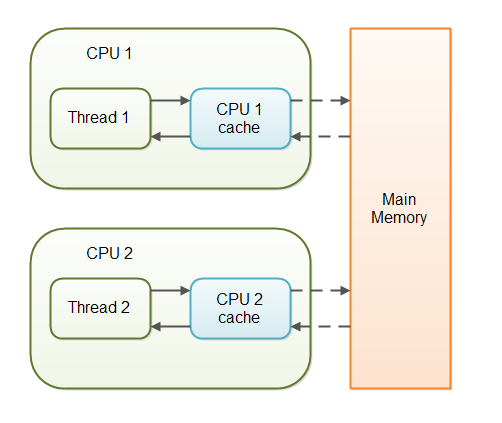
\includegraphics[scale=0.5]{volatile.png}
\end{center}

\subsubsection{Atomic package}
Use this when we are modifying values of variables concurrently. For example, \lstinline{AtomicInteger}, an object representing an int value that may be updated atomically:
\begin{itemize}
    \item \lstinline{int accumulateAndGet(int x, IntBinaryOperator accumulatorFunction)} Atomically updates the current value with the results of applying the given function to the current and given values, returning the updated value.
    \item \lstinline{int addAndGet(int delta)} Atomically adds the given value to the current value.
    \item \lstinline{boolean compareAndSet(int expect, int update)} Atomically sets the value to the given updated value if the current value == the expected value.
    \item \lstinline{int decrementAndGet()} Atomically decrements by one the current value.
    \item \lstinline{double doubleValue()} Returns the value of this AtomicInteger as a double after a widening primitive conversion.
    \item \lstinline{float floatValue()} Returns the value of this AtomicInteger as a float after a widening primitive conversion.
    \item \lstinline{int get()} Gets the current value.
    \item \lstinline{int getAndAccumulate(int x, IntBinaryOperator accumulatorFunction)} Atomically updates the current value with the results of applying the given function to the current and given values, returning the previous value.
    \item \lstinline{int getAndAdd(int delta)} Atomically adds the given value to the current value.
    \item \lstinline{int getAndDecrement()} Atomically decrements by one the current value.
    \item \lstinline{int getAndIncrement()} Atomically increments by one the current value.
    \item \lstinline{int getAndSet(int newValue)} Atomically sets to the given value and returns the old value.
    \item \lstinline{int getAndUpdate(IntUnaryOperator updateFunction)} Atomically updates the current value with the results of applying the given function, returning the previous value.
    \item \lstinline{int incrementAndGet()} Atomically increments by one the current value.
    \item \lstinline{int intValue()} Returns the value of this AtomicInteger as an int.
    \item \lstinline{void lazySet(int newValue)} Eventually sets to the given value.
    \item \lstinline{long longValue()} Returns the value of this AtomicInteger as a long after a widening primitive conversion.
    \item \lstinline{void set(int newValue)} Sets to the given value.
    \item \lstinline{String toString()} Returns the String representation of the current value.
    \item \lstinline{int updateAndGet(IntUnaryOperator updateFunction)} Atomically updates the current value with the results of applying the given function, returning the updated value.
    \item \lstinline{boolean weakCompareAndSet(int expect, int update)} Atomically sets the value to the given updated value if the current value == the expected value.
\end{itemize}
Usage in threads:\\
    \lstinline|class Incrementer extends Thread {|\\
    \lstinline|  public void run () {|\\
    \lstinline|      myAtomicInteger.incrementAndGet();|\\
    \lstinline|  }|\\
    \lstinline|}|

\subsubsection{Intrinsic locking: Synchronized methods}
\paragraph {Synchronized methods} At its simplest level, a block of code that is marked as synchronized in Java tells the JVM: ``only let one thread in here at a time''. Marking a method as \lstinline{synchronized} makes the compiler append instructions to acquire the lock on the specified object before executing the code, and release it afterwards (either because the code finishes normally or abnormally). Intrinsic locks are reentrant.

\paragraph{Synchronized blocks}
Every Java \lstinline{Object} can implicitly act as a lock for purposes of synchronization, using the \lstinline{synchronized} block:\\
    \lstinline|synchronized (lock) {|\\
    \lstinline|  //Access shared state guarded by lock|\\
    \lstinline|}|\\
NOTE: Always be careful of the \textbf{locking policy} and be aware of what you are locking. If you lock on two different objects when what you really wanted was to synchronize on the same object, then the locking is useless.

\subsubsection{Private locking: ReentrantLock}
\lstinline|class Withdrawer extends Thread {|\\
\lstinline|  public void run () {|\\
\lstinline|    reentrantMutex.lock();|\\
\lstinline|    if (saving >= 1000) {|\\
\lstinline|      saving = saving - 1000;|\\
\lstinline|      cash = cash + 1000;|\\
\lstinline|    }|\\
\lstinline|    reentrantMutex.unlock();|\\
\lstinline|  }|\\
\lstinline|}|

\paragraph{Usage and Conditions} When a thread requests a lock that is already held by another thread, the requesting thread blocks. Also, possible to wait on certain conditions using \lstinline{Condition c = reentrantMutex.newCondition()} and then using \lstinline{c.await()}, \lstinline{c.awaitInterruptibly()} to cause the current thread to wait until it is signalled or interrupted, and \lstinline{c.signal()} and \lstinline{c.signalAll()} to wake up one/all waiting thread(s) for that particular condition.

\paragraph{tryLock()} Acquires the lock if it is not held by another thread and returns immediately with the value true, setting the lock hold count to one. Even when this lock has been set to use a fair ordering policy, a call to \lstinline{tryLock()} will immediately acquire the lock if it is available, whether or not other threads are currently waiting for the lock. This "barging" behavior can be useful in certain circumstances, even though it breaks fairness. If you want to honor the fairness setting for this lock, then use \lstinline{tryLock(0, TimeUnit.SECONDS)} (acquires the lock if it's available within the given waiting time), which is almost equivalent (it also detects interruption). If the current thread already holds this lock then the hold count is incremented by one and the method returns true. If the lock is held by another thread then this method will return immediately with the value false. Here is an example that uses \lstinline{ReentrantLock} and \lstinline{tryLock()}, to solve the Dining Philosophers' Problem:

\lstinputlisting{src/DiningPhil1.java}

\subsection{Locking Policy}

\subsubsection{How do I make something Thread-safe?}
\begin{enumerate}
    \item Ask, what is the \textbf{Object's state} and what \textbf{constraints} does it have?
        \begin{enumerate}
            \item All mutable variables, if they are all primitive.
            \item All mutable variables + references to other Objects, otherwise.
            \item Reduce this state space by using final variables.
            \item Identify if things like atomicity and encapsulation are required.
        \end{enumerate}
    \item How do I establish and implement the policy for concurrent access to these variables?
        \begin{enumerate}
            \item Guard each mutable variable with one lock.
            \item Guard related variables with the same locks.
            \item Make sure every access of any variable is guarded by the lock according to the policy.
            \item Make sure access of the related variables in the same method is in synchronized block.
            \item Add waiting (and notify) to handle pre-conditions.
        \end{enumerate}
    \item Can you \textbf{extend another class} that's already known to be Thread-safe?
        \begin{enumerate}
            \item If there exists such a class supporting most to all of the needed operations.
            \item If you know the locking policy of that class.
            \item \textbf{More fragile than modifying the class directly}, because the implementation of the synchronization policy is now distributed over multiple, separately maintained source files.
        \end{enumerate}
    \item If you don't have access to such a class, can you use \textbf{Client-side locking}?
        \begin{enumerate}
            \item If we know the client's locking policy. Client-side locking is when we outsource the locking and unlocking to the program that is requesting the resource.
            \item The following example is \textbf{wrong}:\\
                \lstinline|public class ListHelper<E> {|\\
                \lstinline|  public java.util.List<E> list = Collections.synchronizedList(new ArrayList<E>());|\\\\
                \lstinline|  public synchronized boolean putIfAbsent(E x) {|\\
                \lstinline|    boolean absent = !list.contains(x);|\\
                \lstinline|    if (absent) {|\\
                \lstinline|        list.add(x);|\\
                \lstinline|    }|\\
                \lstinline|    return absent;|\\
                \lstinline|  }|\\
                \lstinline|}|
            \item Here, the method \lstinline{putIfAbsent()} is \lstinline{synchronized}, but on the superclass instead of on the list. Multiple threads can still modify the list through other methods without acquiring the lock on the list object. The solution is to wrap the contents of the method with the block \lstinline{synchronized (list)} instead.
            \item In general, \textbf{Client-side locking is even more fragile} than extending the class because it distributes the locking policy for a class into classes that are totally unrelated.
        \end{enumerate}
    \item \textbf{Composition:} Or I can make a \textbf{data structure wrapper} around \lstinline{List<E>}, for example, where \textbf{everything} is \lstinline{synchronized}. That way I don't need to care if \lstinline{List<E>} is Thread-safe or not, I can just interface with it using my \lstinline{synchronized} methods.
        \begin{enumerate}
            \item Yes, but then the whole data structure takes a performance hit. Imagine if every method accessing, reading, writing, modifying a data structure is made \lstinline{synchronized}, and you have say, thousands of threads trying to do operations on that structure. It's going to slow down quite a bit.
        \end{enumerate}
    \item Are the instances confined?
        \begin{enumerate}
            \item Objects mustn't escape their scope. Escaping includes public variables lying around, methods locking on wrong objects, etc.
            \item Things such as \lstinline{public int topOfStack} shouldn't be lying around in public. Some other program can modify it directly even without using the thread-safe method that you went through great pains to implement.
            \item How to confine? Use \lstinline{private}, make variables local, confine variables to the specific threads if they are not supposed to be shared.
        \end{enumerate}
\end{enumerate}

\subsection{Java's Concurrency Library}
Synchronized Collections, Concurrent Collections, and Synchronizers.

\subsubsection{Synchronized collections}
\paragraph{Why are \lstinline{Vector} and \lstinline{Hashtable} deprecated?} All of the get(), set() methods are synchronized, so you can't have fine grained control over synchronization. Vector is essentially an early ArrayList that has all its methods synchronized, and Hashtable is an early Hashmap that's synchronized whereas the new HashMap is not. They are not efficient if the data structure starts getting large and because of using \lstinline{synchronized} everywhere they slow down quite a bit.

\paragraph{Internal fail-fast using Iterators} When you do \lstinline{for (Object obj : objList)} where \lstinline{objList} is a \lstinline{List<Object>}, internally, javac generates code that uses an Iterator, repeatedly calling hasNext and next to iterate the list. If the Collection will be changed while some thread is traversing over it using Iterator, the iterator.next() will throw ConcurrentModificationException (an int variable modCount is defined: modCount provides the number of times list size has been changed. modCount value is used in every next() call to check for any modifications in a function checkForComodification()). Therefore you have to lock either when the specific method to modify is called, or before the entire process of iteration, depending on the specification. But this is bad because locking the entire data structure removes the benefits of multithreading. One alternative is to clone the collection, lock and iterate the copy.

\subsubsection{Java 5.0: Concurrent collections}
\paragraph{ConcurrentHashMap} ConcurrentHashMap uses \textbf{lock striping}. An array of 16 locks, with each lock guarding $\dfrac{1}{16}$ of the buckets (bucket N is guarded by lock (N\%16)). The iterators returned by ConcurrentHashMap are weakly consistent (i.e., it is OK to modify the collection while iterating through it) instead of fail-fast, and it cannot be locked for exclusive access. Useful methods in ConcurrentHashMap:
\begin{itemize}
    \item \lstinline{void clear()} Removes all of the mappings from this map.
    \item \lstinline{V computeIfAbsent(K key, Function<? super K,? extends V> mappingFunction)} If the specified key is not already associated with a value, attempts to compute its value using the given mapping function and enters it into this map unless null.
    \item \lstinline{V computeIfPresent(K key, BiFunction<? super K,? super V,? extends V> remappingFunction)} If the value for the specified key is present, attempts to compute a new mapping given the key and its current mapped value.
    \item \lstinline{V get(Object key)} Returns the value to which the specified key is mapped, or null if this map contains no mapping for the key.
    \item \lstinline{V put(K key, V value)} Maps the specified key to the specified value in this table.
    \item \lstinline{V putIfAbsent(K key, V value)} If the specified key is not already associated with a value, associate it with the given value.
    \item \lstinline{V remove(Object key)} Removes the key (and its corresponding value) from this map.
    \item \lstinline{boolean remove(Object key, Object value)} Removes the entry for a key only if currently mapped to a given value.
    \item \lstinline{V replace(K key, V value)} Replaces the entry for a key only if currently mapped to some value.
    \item \lstinline{boolean replace(K key, V oldValue, V newValue)} Replaces the entry for a key only if currently mapped to a given value.
\end{itemize}
Using ConcurrentHashMap's \lstinline{putIfAbsent()} with FutureTask:\\
    \lstinline|// a ConcurrentHashMap with Integers mapping to Future results|\\
    \lstinline|private final ConcurrentHashMap<Integer, Future<List<Integer>>> results|\\
    \lstinline|             = new ConcurrentHashMap<Integer, Future<List<Integer>>>();|\\
    \lstinline|public List<Integer> service (final int input) throws Exception {|\\\\
    \lstinline|  // the future result of factorization|\\
    \lstinline|  Future<List<Integer>> f;|\\\\
    \lstinline|  // set up the futuretask|\\
    \lstinline|  Callable<List<Integer>> eval = new Callable<List<Integer>>() {|\\
    \lstinline|      public List<Integer> call () throws InterruptedException {|\\
    \lstinline|          return factor(input);|\\
    \lstinline|      }|\\
    \lstinline|  };|\\
    \lstinline|  FutureTask<List<Integer>> ft = new FutureTask<List<Integer>>(eval);|\\\\
    \lstinline|  // execute put if absent, if there was no mapping, will put and|\\
    \lstinline|  // return null. Use f for convenience|\\
    \lstinline|  f = results.putIfAbsent(input, ft);|\\\\
    \lstinline|  // If there was no previous mapping, go execute the FutureTask.|\\
    \lstinline|  if (f == null) {|\\
    \lstinline|      f = ft;|\\
    \lstinline|    ft.run();|\\
    \lstinline|  }|\\
    \lstinline|  return f.get();|\\
    \lstinline|}|

\paragraph{CopyOnWriteArrayList} Use this when you must have \textbf{many threads iterating over the ArrayList}. If you don't need to be iterating over long lists with many threads, there is no need for it. This is a thread-safe variant of ArrayList in which all mutative operations (add, set, and so on) are implemented by making a fresh copy of the underlying array. This is ordinarily too costly, but may be more efficient than alternatives when traversal operations vastly outnumber mutations, and is useful when you cannot or don't want to synchronize traversals, yet need to preclude interference among concurrent threads. \textbf{This array never changes during the lifetime of the iterator, so interference is impossible} and the iterator is guaranteed not to throw ConcurrentModificationException. The iterator will not reflect additions, removals, or changes to the list since the iterator was created. All write operations are protected by the same lock and read operations are not protected.

\paragraph{BlockingQueue (Interface)} A BlockingQueue is typically used to have on thread produce objects, which another thread consumes. BlockingQueue uses add() and remove() (which attempt to insert/remove immediately and throw Exceptions if unable), or offer() and poll() (which attempt to insert/remove immediately and return false if unable), or put() and take() (which attempt to insert/remove immediately, and wait/block if necessary till elements/spaces become available). Here is a diagram that illustrates this principle:

\begin{center}
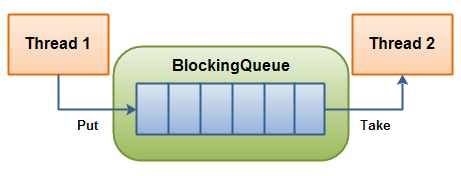
\includegraphics[scale=0.5]{blocking-queue.png}
\end{center}

The producing thread will keep producing new objects and insert them into the queue, until the queue \textbf{reaches some upper bound} on what it can contain. If the blocking queue reaches its upper limit, the \textbf{producing thread is blocked} while trying to insert the new object. It remains blocked until a consuming thread takes an object out of the queue. The consuming thread keeps taking objects out of the blocking queue, and processes them. If the consuming thread tries to take an object out of an empty queue, the \textbf{consuming thread is blocked} until a producing thread puts an object into the queue. An example:\\\\
    \lstinline|class Producer implements Runnable {|\\
    \lstinline| private final BlockingQueue queue;|\\
    \lstinline| Producer(BlockingQueue q) { queue = q; }|\\
    \lstinline| public void run() {|\\
    \lstinline|   try {|\\
    \lstinline|     while (true) { queue.put(produce()); }|\\
    \lstinline|   } catch (InterruptedException ex) { ... handle ...}|\\
    \lstinline| }|\\
    \lstinline| Object produce() { ... }|\\
    \lstinline|}|\\\\
    \lstinline|class Consumer implements Runnable {|\\
    \lstinline| private final BlockingQueue queue;|\\
    \lstinline| Consumer(BlockingQueue q) { queue = q; }|\\
    \lstinline| public void run() {|\\
    \lstinline|   try {|\\
    \lstinline|     while (true) { consume(queue.take()); }|\\
    \lstinline|   } catch (InterruptedException ex) { ... handle ...}|\\
    \lstinline| }|\\
    \lstinline| void consume(Object x) { ... }|\\
    \lstinline|}|\\\\
    \lstinline|class Setup {|\\
    \lstinline| void main() {|\\
    \lstinline|   BlockingQueue q = new SomeQueueImplementation();|\\
    \lstinline|   Producer p = new Producer(q);|\\
    \lstinline|   Consumer c1 = new Consumer(q);|\\
    \lstinline|   Consumer c2 = new Consumer(q);|\\
    \lstinline|   new Thread(p).start();|\\
    \lstinline|   new Thread(c1).start();|\\
    \lstinline|   new Thread(c2).start();|\\
    \lstinline| }|\\
    \lstinline|}|

\paragraph{FutureTask} FutureTask constructors can accept either Runnable or Callable. Runnable and Callable interfaces are designed to represent thread-executable tasks. Why use Callable? A Callable needs to implement call() method while a Runnable needs to implement run() method. A Callable can return a value but a Runnable cannot. A Callable can throw checked exception but a Runnable cannot. FutureTasks are a cancellable asynchronous computation.\\\\
This class provides a base implementation of Future, with methods to start and cancel a computation, query to see if the computation is complete, and retrieve the result of the computation. The result can only be retrieved when the computation has completed; the get methods will block if the computation has not yet completed. Once the computation has completed, the computation cannot be restarted or cancelled (unless the computation is invoked using runAndReset()). A FutureTask can be used to wrap a Callable or Runnable object. \textbf{Because FutureTask implements Runnable, a FutureTask can be submitted to an Executor (or Thread!) for execution}. In addition to serving as a standalone class, this class provides protected functionality that may be useful when creating customized task classes. Methods are as follows:
\begin{itemize}
    \item \lstinline{boolean cancel(boolean mayInterruptIfRunning)} Attempts to cancel execution of this task.
    \item \lstinline{protected void done()} Protected method invoked when this task transitions to state isDone (whether normally or via cancellation).
    \item \lstinline{V get()} Waits if necessary for the computation to complete, and then retrieves its result. 
    \item \lstinline{V get(long timeout, TimeUnit unit)} Waits if necessary for at most the given time for the computation to complete, and then retrieves its result, if available.
    \item \lstinline{boolean isCancelled()} Returns true if this task was cancelled before it completed normally.
    \item \lstinline{boolean isDone()} Returns true if this task completed.
    \item \lstinline{void run()} Sets this Future to the result of its computation unless it has been cancelled.
    \item \lstinline{protected boolean runAndReset()} Executes the computation without setting its result, and then resets this future to initial state, failing to do so if the computation encounters an exception or is cancelled.
    \item \lstinline{protected void set(V v)} Sets the result of this future to the given value unless this future has already been set or has been cancelled.
\end{itemize}

\subsubsection{Synchronizers}
A synchronizer is an object that coordinates the control flow of threads based on its state.

\paragraph{Semaphore} Semaphores are counters that increment/decrement through acquire() and release(). A binary semaphore acts as a mutex. A counting semaphore acts as a set of N permits.

\paragraph{CyclicBarrier} The java.util.concurrent.CyclicBarrier class is a synchronization mechanism that can synchronize threads progressing through some algorithm. In other words, it is a barrier that all threads must wait at, until all threads reach it, before any of the threads can continue. The threads wait for each other by calling the await() method on the CyclicBarrier. Once N threads are waiting at the CyclicBarrier, all threads are released and can continue running. Here is a diagram illustrating that:

\begin{center}
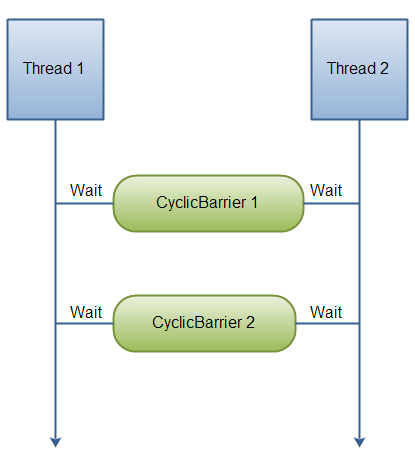
\includegraphics[scale=0.5]{cyclic-barrier.png}
\end{center}

If a timeout is required, \lstinline{barrier.await(N, TimeUnit.SECONDS)} can be used. A thread is released after N seconds even if not all threads have reached the Barrier. The waiting threads waits at the CyclicBarrier until either:
\begin{itemize}
    \item The last thread arrives (calls await()).
    \item The thread is interrupted by another thread (another thread calls its interrupt() method).
    \item Another waiting thread is interrupted.
    \item Another waiting thread times out while waiting at the CyclicBarrier.
    \item The \lstinline{CyclicBarrier.reset()} method is called by some external thread.
\end{itemize}

\paragraph{CountDownLatch} CountDownLatch is a concurrency construct that allows one or more threads to wait for a given set of operations to complete. A CountDownLatch is initialized with a given count. This count is decremented by calls to the countDown() method. Threads waiting for this count to reach zero can call one of the await() methods. Calling await() blocks the thread until the count reaches zero. Below is a simple example. After the Decrementer has called countDown() 3 times on the CountDownLatch, the waiting Waiter is released from the await() call.

\lstinputlisting{src/CDLDemo.java}

\paragraph{Phaser} When to use Phaser (as compared to CyclicBarrier or CountDownLatch): When you don't know the number of threads before run time. That is, when the number of threads vary depending on run time. To give an analogy, consider an university admission: you can have 1000 students register in one year and maybe 800 in another. You only know how many students register when you open the admission portal. CyclicBarrier and CountDownLatch is more suited for applications when you know the number of registered threads before run time. An analogy would be an examination setting where the number of exam takers is known before the exam. What is arriving and waiting (methods arrive(), awaitAdvance() and arriveAndAwaitAdvance())? The notion of arrival is separate from the notion of waiting. Consider this analogy of a theme park ride: after you registered for the ride, you are given a queue number after arrival. You can play other rides before your queue number starts. You eventually return to the first ride and await the ride to start.
\begin{itemize}
    \item \textbf{Registration}. Unlike the case for other barriers, the number of parties registered to synchronize on a phaser may vary over time. Tasks may be registered at any time (using methods register(), bulkRegister(int), or forms of constructors establishing initial numbers of parties), and optionally deregistered upon any arrival (using arriveAndDeregister()). As is the case with most basic synchronization constructs, registration and deregistration affect only internal counts; they do not establish any further internal bookkeeping, so tasks cannot query whether they are registered. (However, you can introduce such bookkeeping by subclassing this class.)
    \item \textbf{Synchronization}. Like a CyclicBarrier, a Phaser may be repeatedly awaited. Method arriveAndAwaitAdvance() has effect analogous to CyclicBarrier.await. Each generation of a phaser has an associated phase number. The phase number starts at zero, and advances when all parties arrive at the phaser, wrapping around to zero after reaching Integer.MAX\_VALUE. The use of phase numbers enables independent control of actions upon arrival at a phaser and upon awaiting others, via two kinds of methods that may be invoked by any registered party:
    \item \textbf{Arrival}. Methods arrive() and arriveAndDeregister() record arrival. These methods do not block, but return an associated arrival phase number; that is, the phase number of the phaser to which the arrival applied. When the final party for a given phase arrives, an optional action is performed and the phase advances. These actions are performed by the party triggering a phase advance, and are arranged by overriding method onAdvance(int, int), which also controls termination. Overriding this method is similar to, but more flexible than, providing a barrier action to a CyclicBarrier.
    \item \textbf{Waiting}. Method awaitAdvance(int) requires an argument indicating an arrival phase number, and returns when the phaser advances to (or is already at) a different phase. Unlike similar constructions using CyclicBarrier, method awaitAdvance continues to wait even if the waiting thread is interrupted. Interruptible and timeout versions are also available, but exceptions encountered while tasks wait interruptibly or with timeout do not change the state of the phaser. If necessary, you can perform any associated recovery within handlers of those exceptions, often after invoking forceTermination. Phasers may also be used by tasks executing in a ForkJoinPool, which will ensure sufficient parallelism to execute tasks when others are blocked waiting for a phase to advance.
    \item \textbf{Termination}. A phaser may enter a termination state, that may be checked using method isTerminated(). Upon termination, all synchronization methods immediately return without waiting for advance, as indicated by a negative return value. Similarly, attempts to register upon termination have no effect. Termination is triggered when an invocation of onAdvance returns true. The default implementation returns true if a deregistration has caused the number of registered parties to become zero. As illustrated below, when phasers control actions with a fixed number of iterations, it is often convenient to override this method to cause termination when the current phase number reaches a threshold. Method forceTermination() is also available to abruptly release waiting threads and allow them to terminate.
    \item \textbf{Tiering}. Phasers may be tiered (i.e., constructed in tree structures) to reduce contention. Phasers with large numbers of parties that would otherwise experience heavy synchronization contention costs may instead be set up so that groups of sub-phasers share a common parent. This may greatly increase throughput even though it incurs greater per-operation overhead. In a tree of tiered phasers, registration and deregistration of child phasers with their parent are managed automatically. Whenever the number of registered parties of a child phaser becomes non-zero (as established in the Phaser(Phaser,int) constructor, register(), or bulkRegister(int)), the child phaser is registered with its parent. Whenever the number of registered parties becomes zero as the result of an invocation of arriveAndDeregister(), the child phaser is deregistered from its parent.
    \item \textbf{Monitoring}. While synchronization methods may be invoked only by registered parties, the current state of a phaser may be monitored by any caller. At any given moment there are getRegisteredParties() parties in total, of which getArrivedParties() have arrived at the current phase (getPhase()). When the remaining (getUnarrivedParties()) parties arrive, the phase advances. The values returned by these methods may reflect transient states and so are not in general useful for synchronization control. Method toString() returns snapshots of these state queries in a form convenient for informal monitoring. This also differs from CyclicBarrier or CountDownLatch where both arriving and waiting is combined. 
\end{itemize}
Using \lstinline{Phaser} to dynamically wait for N number of threads:\\\\
\lstinline|void runTasks(List<Runnable> tasks) {|\\
\lstinline|  final Phaser phaser = new Phaser(1); // "1" to register self|\\
\lstinline|  // create and start threads|\\
\lstinline|  for (final Runnable task : tasks) {|\\
\lstinline|   phaser.register();|\\
\lstinline|   new Thread() {|\\
\lstinline|     public void run() {|\\
\lstinline|       phaser.arriveAndAwaitAdvance(); // await all creation|\\
\lstinline|       task.run();|\\
\lstinline|     }|\\
\lstinline|   }.start();|\\
\lstinline|  }|\\\\
\lstinline|  // allow threads to start and deregister self|\\
\lstinline|  phaser.arriveAndDeregister();|\\
\lstinline|}|
 
\begin{center}
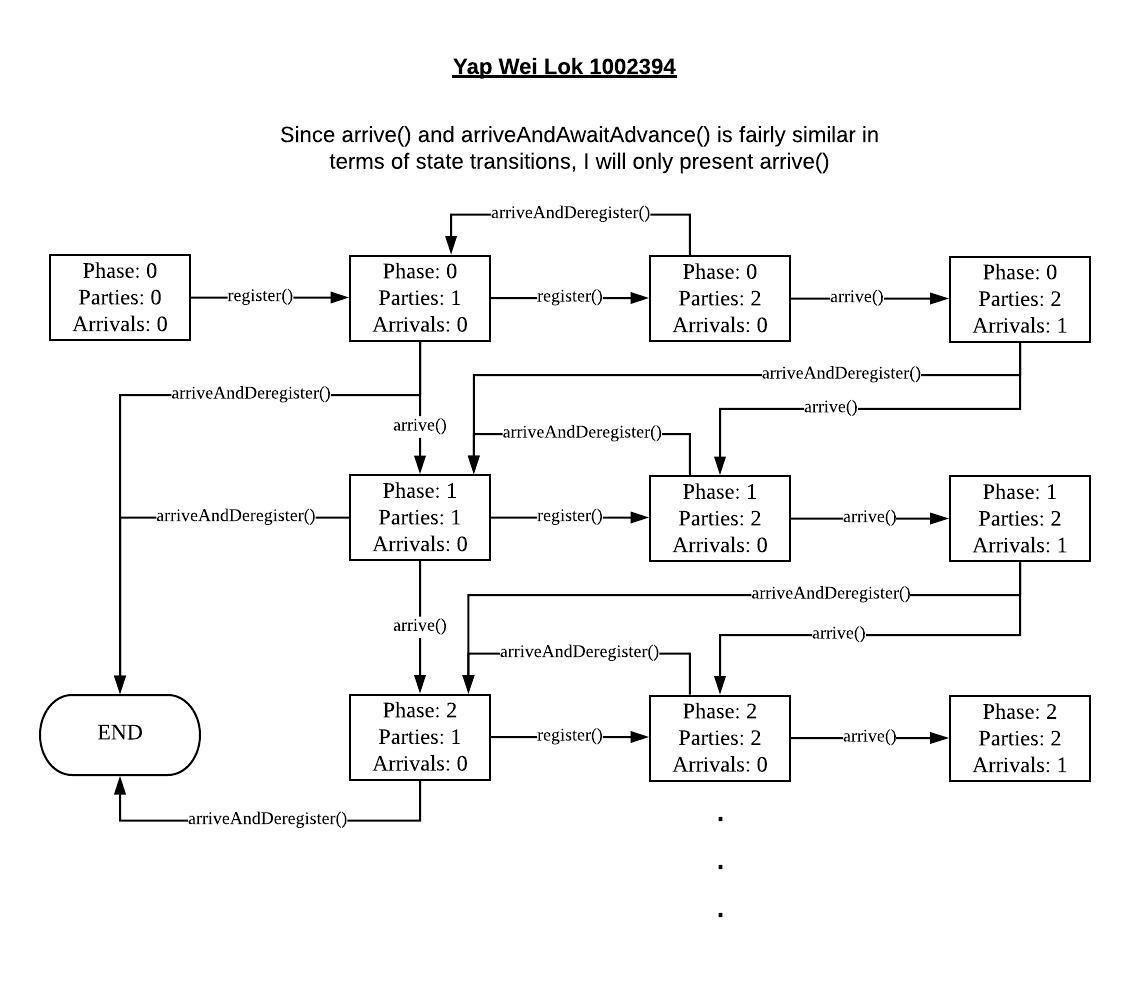
\includegraphics[scale=0.8]{phaser.jpg}
\end{center}

\section{Testing Concurrent Programs}
\begin{enumerate}
    \item Create an object of the class, call its methods (in different sequences with different inputs) and assert post-conditions and invariants. 
    \item Set up multiple threads performing operations over some amount of time and then somehow test that nothing went wrong. Mind that the test programs are concurrent programs too! It’s best if checking the test property does not require any synchronization.
    \item How do we test that everything put into the buffer comes out of it and that nothing else does, assuming there are multiple producers and consumers?
    \begin{enumerate}
        \item A naïve approach: maintain a ``shadow'' list and assert that the buffer is consistent with the ``shadow'' list
        \item Use a checksum function would be better
    \end{enumerate}
    \item Some test data should be generated randomly.
    \item Random number generator can create couplings between classes and timing artifacts because most random number generator classes are thread-safe and therefore introduce additional synchronization.
    \item Often we need to generate more scheduling, especially if the time to completion is small. We can do things like:
        \begin{enumerate}
            \item Test with more active threads than CPUs.
            \item Testing with different processor counts, operating systems, and processor architectures.
            \item Encourage context switching using Thread.yield() or Thread.sleep.
        \end{enumerate}
    \item Or just use tools (Team Explorer, Codeclimate, Coverity Scan, ...).
\end{enumerate}

\section{Optimization in Concurrency}
\subsection{Assigning Threads for Tasks}
\subsubsection{One thread per task}
The idea is to create a new thread for every task that we need to execute. This is responsive, but you end up with a huge number of threads in real-world applications (e.g. large web servers). You gain parallel processing, but the code has to be thread-safe. Susceptible to DDoS because of unbound thread creation. Thread creation and tear down involves the JVM and OS. For lots of lightweight threads this is not very efficient. Active Threads consume extra memory, for instance to provide for a thread stack. If there are less CPU's than threads, some threads sit idle, consuming memory. There is a limit on how many threads you can have concurrently. If you hit this limit your program will most likely become unstable.

\subsection{Thread Pooling}
Using worker threads minimizes the overhead due to thread creation. Thread objects use a significant amount of memory, and in a large-scale application, allocating and deallocating many thread objects creates a significant memory management overhead. One common type of thread pool is the fixed thread pool. This type of pool always has a specified number of threads running; if a thread is somehow terminated while it is still in use, it is automatically replaced with a new thread. Tasks are submitted to the pool via an internal queue, which holds extra tasks whenever there are more active tasks than threads. By properly tuning the size of the thread pool, you can have enough threads to keep the processors busy while not having so many that your application runs out of memory or thrashes (screws up the garbage collector when a large number of temporary objects are created in very short intervals) due to competition among threads for resources.

\subsubsection{Executor and ExecutorService}
Delegation. The \textbf{Executor} (Interface) framework offers flexible thread pool management, provides a standard means of decoupling task submission from task execution. Executor just executes stuff you give it, while ExecutorService adds startup, shutdown, and the ability to wait for and look at the status of jobs you've submitted for execution on top of Executor (which it extends); ExecutorService offers \textbf{submit(), invoke() and shutdown() functions}. Using shutdown() will just tell the executor service that it can't accept new tasks, but the already submitted tasks continue to run. There's also shutdownNow() which will do the same AND will try to cancel the already submitted tasks by interrupting the relevant threads. Note that if your tasks ignore the interruption, shutdownNow() will behave exactly the same way as shutdown().

\subsubsection{Thread pool types}
\begin{itemize}
    \item \textbf{newFixedThreadPool}, Fixed-size thread pool; creates threads as tasks are submitted, up to the maximum pool size and then attempts to keep the pool size constant
    \item \textbf{newCachedThreadPool}, Boundless, but the pool shrinks and grows when demand dictates so
    \item \textbf{newSingleThreadExecutor}, A single worker thread to process tasks, sequentially according to the order imposed by the task queue
    \item \textbf{newScheduledThreadPool}, A fixed-size thread pool that supports delayed and periodic task execution.
\end{itemize}

\subsubsection{Execution policy and Optimizing the thread pool}
\paragraph{So when do I thread pool?} Thread pools work best when \textbf{tasks are homogeneous and independent} (Dependency between tasks in the pool creates constraints on the execution policy which might result in deadlock, liveness, etc.).\\
\\
The optimal pool size, $S_{pool}$ is:

\begin{equation}
    S_{pool} = N_{CPU} \cdot u_{CPU} \cdot \left(1 + \dfrac{t_{wait}}{t_{compute}}\right)
\end{equation}

Where $N_{CPU}$ is the number of CPUs, $u_{CPU}$ is the target CPU utilization $\epsilon \ (0,1)$, and $\dfrac{t_{wait}}{t_{compute}}$ is the ratio of waiting time to compute time. Decoupling submission from execution is that it lets you specify the execution policy for a given class of tasks:

\begin{itemize}
    \item In what thread will tasks be executed?
    \item In what order should tasks be executed (FIFO)?
    \item How many tasks may execute concurrently?
    \item How many tasks may be queued pending execution?
    \item If a task has to be rejected because the system is overloaded, which task should be selected and how the application be notified?
    \item What actions should be taken before or after executing a task?
\end{itemize}

\paragraph{Alternative ways of tuning} Other resources that can contribute to sizing constraints are memory, file handles, socket handles, database connections, etc. Add up how much of those resources each task requires and divide that into the total quantity available. Alternatively, the size of the thread pool can be tuned by running the application using different pool sizes and observing the level of CPU and other resource utilization.

\paragraph{Writing the code} The execution policy is \textbf{defined in the execute() method of your concrete Executor class}. Typically, the Executor is set up in this fashion:
\begin{enumerate}
    \item \lstinline|private static final int NTHREADS = 50;|
	\item \lstinline|private static final Executor exec = Executors.newFixedThreadPool(NTHREADS);|
	\item \lstinline|Runnable task = new Runnable () { public void run() { //something }};|
	\item \lstinline|exec.execute(task);|
\end{enumerate}

\subsection{Parallelization}
\subsubsection{How to maximize performance by defining tasks?}

\begin{center}
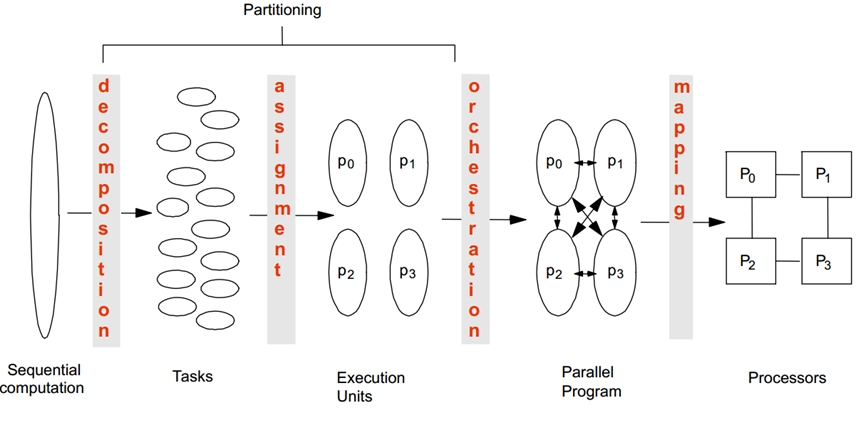
\includegraphics[scale=0.7]{img/parallelization.png}    
\end{center}

\begin{enumerate}
    \item Decomposition: Break up the computation into “self-contained” tasks to be divided among processes. Tasks should be medium-sized. If too small, the ratio of useful work vs overhead becomes small. If too big, the number of tasks available at a time is upper bound on achievable speedup. Tasks may become available dynamically!
    \item Assignment: Specify mechanism to divide work among cores. We may want to balance the amount of work for each core and reduce communication between the threads and apply Well-known design patterns.
    \item Orchestration and Mapping: Figure out what kind of communication is needed between each pair of threads. Less communication is better: preserve locality of data! Schedule the threads to satisfy tasks' dependencies and use Executor to manage the thread pool.
\end{enumerate}

\paragraph{A note on dependency} Dependency is defined, by Bernstein's condition, if two tasks cannot run in parallel because of some action or output that preceeds the input of the next task.

\paragraph{What if you don't want to use Executor?} Then we need to consider the number of execution units platform will support (we have a maximum number of threads!), and the cost of sharing information among execution units. In this case, optimize to do things like DFS in parallel.


\subsection{Design Patterns for Parallelization}

\subsubsection{Pattern 1: Single Program Multiple Data (SPMD)}
All threads/processes run the same program, operating on different data. This model is particularly appropriate for problems with a regular, predictable communication pattern. MATLAB supports SPMD blocks. Often adopted for GPU programming. In the cohort exercise we split an integration task by assigning threads for different intervals.

\subsubsection{Pattern 2: Loop Parallelism}
If we need to loop from $i = 0$ to $i < 3000$, Thread A can loop from 0 to 999, B from 1000 to 1999, C from 2000 to 2999.

\subsubsection{Pattern 3: Master-Worker Pattern}
A master thread/process divides a problem into several sub-problems and dispatches them to several worker processes.

\subsubsection{Pattern 4: Fork-Join Pattern}
Tasks can create more tasks! Tasks manage other tasks according to their relationship. Parent task creates new tasks (fork) then waits until they complete (join) before continuing on with the computation. For example, \textbf{How to parallelize BFS?} Nodes of the same hop-distance (level) from the root can be visited in parallel by child threads:

\begin{center}
    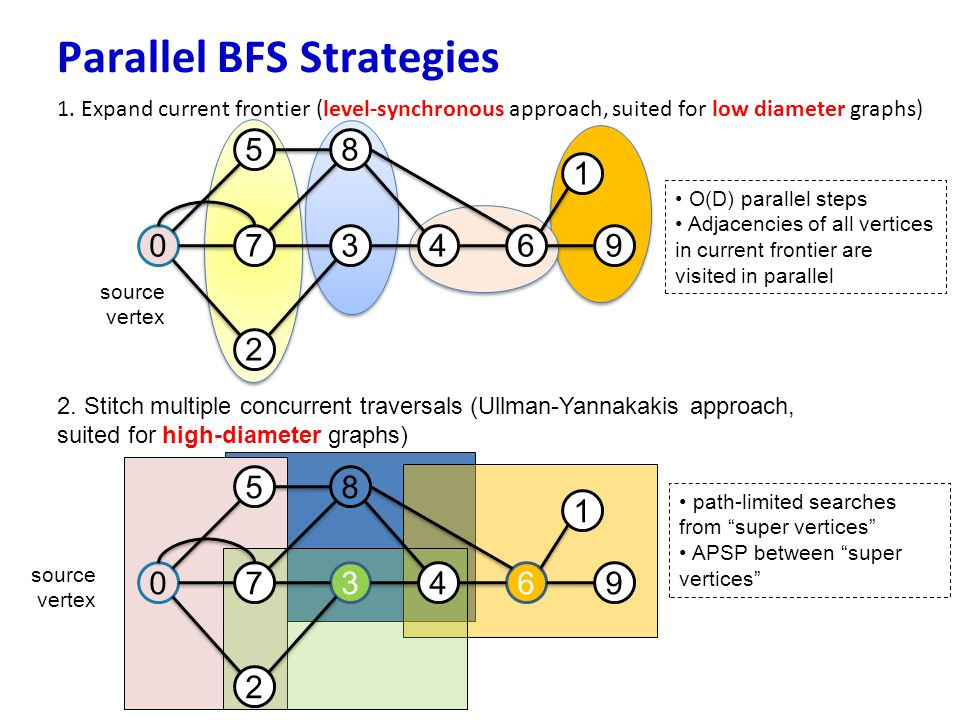
\includegraphics[scale=0.4]{img/parallel-bfs.jpg}
\end{center}

\subsection{Dealing with Limitations in Concurrency}
\subsubsection{Limits: Amdahl's law}
Amdahl's law says that on a machine with N processors, and $F$ is the fraction of the code that must be executed serially we can achieve a speed up of at most:
\begin{equation}
    speedup \leq \frac{1}{F+\frac{1-F}{N}}
\end{equation}
All concurrent programs have some degree of \textbf{serialization}.

\subsubsection{The cost of using threads}
\textbf{Context switching} requires saving the context of the currently running thread and restoring the execution context of the newly scheduled thread. \textbf{Cache misses} are deadly, cost about 5,000 to 10,000 clock cycles. In memory synchronization, memory barriers inhibit compiler optimization.

\subsubsection{The cost of using locks}
\paragraph {Locks naturally induce serialization.} A thread with the lock may be delayed (due to a page fault, scheduling delay, etc.). One thread at a time can acquire locks and execute critical section code. Performance takes a hit if many threads are vying for the lock, or the locks are being held for long periods of time. Locking is simply a heavyweight mechanism for simple operations like count++. So how do we fix this?\\\\
\lstinline|public synchronized boolean userLocationMatches (String name, String regexp) {|\\
\lstinline|  String key = "users." + name + ".location";|\\
\lstinline|  String location = attributes.get(key);|\\\\
\lstinline|  if (location == null) {|\\
\lstinline|    return false;|\\
\lstinline|  }|\\
\lstinline|  else {|\\
\lstinline|    return Pattern.matches(regexp, location);|\\
\lstinline|  }|\\
\lstinline|}|\\
\paragraph{Refactor!} Here, the entire method is synchronized, leading to serialization when there are many threads trying to get the key. But we notice that the rest of the method, other than \lstinline{attributes.get()} \textbf{doesn't} need to be synchronized! We can effectively reduce the serialization to:\\\\
\lstinline|public boolean userLocationMatches (String name, String regexp) {|\\
\lstinline|  String key = "users." + name + ".location";|\\
\lstinline|  String location;|\\
\lstinline|  synchronized(this) {|\\
\lstinline|    location = attributes.get(key)|\\
\lstinline|  }|\\
\lstinline|  if (location == null) {|\\
\lstinline|    return false;|\\
\lstinline|  }|\\
\lstinline|  else {|\\
\lstinline|    return Pattern.matches(regexp, location);|\\
\lstinline|  }|\\
\lstinline|}|\\
\paragraph{Or even better, delegate concurrency to ConcurrentHashMap.} We assume there exists a new \lstinline{private final Map<String, String> attributes = new ConcurrentHashMap<String, String>()}, eliminating the need for manual locking:\\\\
\lstinline|public boolean userLocationMatches (String name, String regexp) {|\\
\lstinline|  String key = "users." + name + ".location";|\\
\lstinline|  String location = attributes.get(key); // the get method in CHM is already thread-safe|\\\\
\lstinline|  if (location == null) {|\\
\lstinline|    return false;|\\
\lstinline|  }|\\
\lstinline|  else {|\\
\lstinline|    return Pattern.matches(regexp, location);|\\
\lstinline|  }|\\
\lstinline|}|\\\\
In general, we can improve performance by \textbf{locking on different objects} to reduce the time and demand for locks. But of course these have to make sense and must still be thread-safe. We can also do \textbf{lock striping} like in the case of \lstinline{ConcurrentHashMap}. Even more alternatives exist in the form of \textbf{read-write locks} (more than one reader can access the shared resource concurrently, but writers must acquire the lock exclusively), \textbf{immutable objects} and \textbf{atomic variables}.

\subsubsection{Using Future}
Place time limits on tasks by using \lstinline{Future.get(long timeout, TimeUnit unit)} to time out.\\
\lstinputlisting{src/FutureRenderer2.java}

\subsection{Non-Blocking Synchronization}
Very simplified, the idea is to keep checking if some other thread has already modified your stuff in an atomic way. An algorithm is called non-blocking if failure or suspension of any thread cannot cause failure or suspension of another thread. Non-blocking algorithms are immune to deadlock (though, in unlikely scenarios, may exhibit livelock or starvation) Examples: Stacks (Treiber's), queues, hash tables, etc.

\subsubsection{Hardware support}
\paragraph{Compare-And-Swap} CAS has three operands: a memory location V, the expected old value A, and the new value B. CAS updates V to the new value B, but only if the value in V matches the expected old value A; otherwise, it does nothing. In either case, it returns the value currently in V. CAS is supported in atomic variable classes.
\paragraph{Example: Non-blocking stack} Java has \lstinline{AtomicReference}, an object reference that may be updated atomically. It has lots of atomic methods like getAndSet(), compareAndSet(), and accumulateAndGet().\\\\
\lstinline|public class ConcurrentStack <E> {|\\
\lstinline|  AtomicReference<Node<E>> top = new AtomicReference<Node<E>>();|\\\\
\lstinline|  public void push(E item) {|\\
\lstinline|    Node<E> newHead = new Node<E>(item);|\\
\lstinline|    Node<E> oldHead;|\\
\lstinline|    do {|\\
\lstinline|      oldHead = top.get();|\\
\lstinline|      newHead.next = oldHead;|\\
\lstinline|    } while (!top.compareAndSet(oldHead, newHead)); //commitment here|\\
\lstinline|  }|\\\\
\lstinline|  public E pop() {|\\
\lstinline|    Node<E> oldHead;|\\
\lstinline|    Node<E> newHead;|\\
\lstinline|    do {|\\
\lstinline|      oldHead = top.get();|\\
\lstinline|      if (oldHead == null)|\\
\lstinline|        return null;|\\
\lstinline|      newHead = oldHead.next;|\\
\lstinline|    } while (!top.compareAndSet(oldHead, newHead)); //commitment here|\\
\lstinline|    return oldHead.item;|\\
\lstinline|  }|\\\\
\lstinline|  private static class Node <E> {|\\
\lstinline|    public final E item;|\\
\lstinline|    public Node<E> next;|\\\\
\lstinline|    public Node(E item) {|\\
\lstinline|      this.item = item;|\\
\lstinline|    }|\\
\lstinline|  }|\\
\lstinline|}|
\paragraph{Example: Non-blocking linked-list}
\begin{center}
    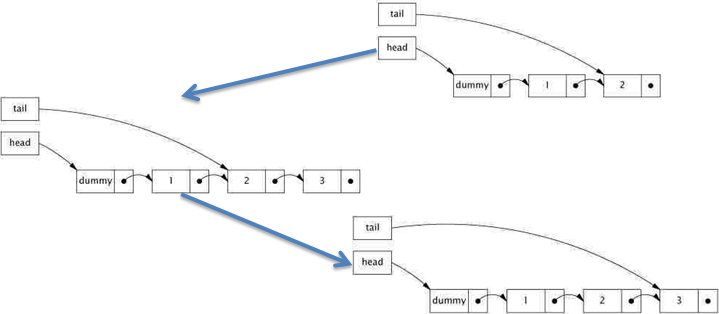
\includegraphics[scale=0.8]{img/nonblockingll.png}
\end{center}
If the queue is in the normal state, tail.next is null. In that case, then we can try and modify it. All pointers are AtomicReferences.
\lstinline|public boolean put(E item) {|\\
\lstinline|  Node<E> newNode = new Node<E>(item, null);|\\
\lstinline|  while (true) {|\\
\lstinline|    Node<E> curTail = tail.get();|\\
\lstinline|    Node<E> tailNext = curTail.next.get();|\\
\lstinline|    if (curTail == tail.get()) { //if this is not true, abort since other some other thread has already modified tail;|\\
\lstinline|      if (tailNext != null) { // if this is true, Queue in intermediate state, advance tail|\\
\lstinline|        tail.compareAndSet(curTail, tailNext);   |\\
\lstinline|      } else {|\\
\lstinline|        // In normal state, try inserting new node|\\
\lstinline|        if (curTail.next.compareAndSet(null, newNode)) { |\\
\lstinline|          // Insertion succeeded, try advancing tail|\\
\lstinline|          tail.compareAndSet(curTail, newNode);|\\
\lstinline|          return true;|\\
\lstinline|        }|\\
\lstinline|      }|\\
\lstinline|    }|\\
\lstinline|  }|\\
\lstinline|}|
\end{document}
